\subsection{Controlled demonstration}

\paragraph{Setup.}
Does accounting for observational uncertainty change which forecast version wins? I start with a controlled case: both versions are centred on the reported value $y$, which isolates the spread dimension---both metrics handle location identically. The setup:

\begin{itemize}
    \item The reported observation is $y = 50$.
    \item The assumed observational uncertainty is $\sigma_\text{rel} = 0.4$ in log-space (the Constructor~3 working default; see \S3 for calibration against the RVI Gumbel model).
    \item Two forecast versions predict the same observation:
    \begin{itemize}
        \item \textbf{Tight (overconfident):} LogNormal($\log y$, $\sigma_\text{tight} = 0.05$)---concentrates nearly all probability mass on a single value, claiming to know the truth precisely.
        \item \textbf{Honest:} LogNormal($\log y$, $\sigma_\text{honest} = 0.4$)---a wider distribution matching the true observational uncertainty.
    \end{itemize}
\end{itemize}

\paragraph{Results.}
Classical CRPS ranks the tight version first: its narrow distribution is closer to the step at $y$ at almost every $z$, and the squared-area integrand is smaller. The reformulated metric, computed against a smooth $F_\text{obs}$ constructed via Constructor~3 ($\sigma_\text{rel} = 0.4$), reverses the ranking: the honest version wins. Figure~\ref{fig:reversal} shows the four scores. The reversal is qualitative, not a numerical artifact. In this baseline case, the reversal is algebraically guaranteed: the Cram\'er distance is an $L^2$ metric, and $\sigma_\text{honest} = \sigma_\text{rel}$ means the honest version's CDF matches $F_\text{obs}$ exactly, which is the minimiser by construction. The substantive question is not \emph{whether} the reversal occurs at the matched parameterisation, but \emph{how far} the honest version can deviate from $F_\text{obs}$ and still beat the overconfident version.

\begin{figure}[h]
    \centering
    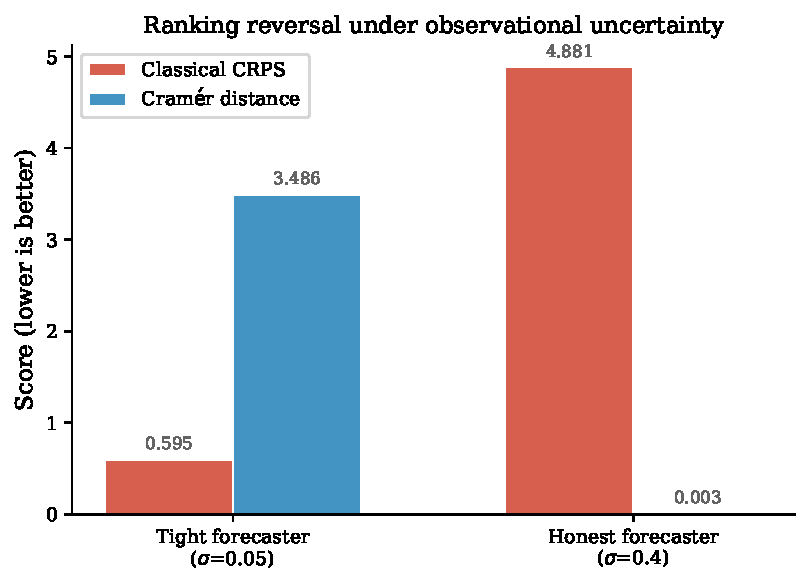
\includegraphics[width=0.7\textwidth]{figures/uncertainty_aware_ranking.pdf}
    \caption{Ranking reversal between two forecast versions on a controlled example. Under classical CRPS the tight (overconfident) version wins; under the Cram\'er-distance reformulation the honest version wins. The reversal is qualitative---the sign of which version is better changes.}
    \label{fig:reversal}
\end{figure}

The reversal does not depend on the honest version exactly matching $F_\text{obs}$: varying $\sigma_\text{honest}$ while holding $\sigma_\text{rel} = 0.4$ fixed, the reversal holds for $\sigma_\text{honest} \in [0.10, \, 0.85]$---the honest version can be $4\times$ too narrow or $2\times$ too wide and still beat the tight version. The reversal disappears when observational uncertainty is small ($\sigma_\text{rel} \leq 0.10$) or when the honest version is extremely wide ($\sigma_\text{honest} \geq 1.0$). Detailed robustness analysis---including constructor comparison, location-error tolerance, and generalisation across distributional families---is in Appendix~\ref{sec:appendix_demo}.

\subsection{Empirical comparison on UCDP conflict data}

\paragraph{Data and design.}
I replicate the controlled demonstration on real observations from the UCDP Georeferenced Event Dataset (GED, data version 24.1, final-coded events; codebook: \citealt{ucdp_codebook}), using best-estimate fatality counts from 2020--2024 aggregated to the PRIO-GRID cell-month level (a $0.5^\circ \times 0.5^\circ$ geographic grid cell observed in a single calendar month, the standard spatiotemporal unit in VIEWS-format evaluations). I pool state-based, non-state, and one-sided violence and retain cell-months with at least one recorded fatality; historical uncertainty is derived from cells with $\geq 3$ active months during 1989--2019. This yields 19{,}397 cell-months from 2{,}065 cells. This sample covers the active-conflict portion of the evaluation space; the roughly 800{,}000 cell-months with zero recorded fatalities are excluded because $F_\text{obs}$ degenerates to a step function at zero and the reformulation reduces to classical CRPS. The results therefore characterise the regime where observational uncertainty is operative, not the full VIEWS evaluation grid.

For each cell-month I construct two forecast versions, both centred on the reported best estimate $y$:
\begin{itemize}
    \item \textbf{Tight:} $\text{LogNormal}(\log y, \, 0.05)$---claims to know the observation precisely.
    \item \textbf{Honest:} $\text{LogNormal}(\log y, \, \hat{\sigma}_\text{cell})$---where $\hat{\sigma}_\text{cell} = \sqrt{\log(1 + \text{CV}^2)}$ is derived from the cell's historical coefficient of variation. Median $\hat{\sigma}_\text{cell} = 0.97$; interquartile range $[0.81, 1.16]$; clipped to $[0.1, 2.0]$ (affecting 1.1\% of cell-months).
\end{itemize}
I score both under classical CRPS and the Cram\'er-distance reformulation with Constructor~3 ($\sigma_\text{rel} = 0.4$).

\paragraph{Results.}
Under classical CRPS the tight version wins in 100\% of cell-months---a direct consequence of both versions being centred on $y$ and CRPS's well-known preference for concentration. Under the Cram\'er-distance reformulation, the ranking reverses in 39\% of cell-months overall.\footnote{The reversal rate is sensitive to $\sigma_\text{rel}$: at $\sigma_\text{rel} = 0.3$ it drops to 12.6\%; at $\sigma_\text{rel} = 0.5$ it rises to 67.7\%.} The reversal rate depends sharply on forecast uncertainty: for cells with moderate uncertainty ($\hat{\sigma}_\text{cell} \leq 0.8$; $n = 4{,}716$), the honest version wins in \emph{every} cell-month. For cells with very high uncertainty ($\hat{\sigma}_\text{cell} > 1.0$; $n = 8{,}902$), the honest version is too wide and loses---exactly the regime identified in the controlled demonstration. Figure~\ref{fig:real_data} shows the reversal rate by uncertainty regime and the score-difference distribution.

\begin{figure}[h]
    \centering
    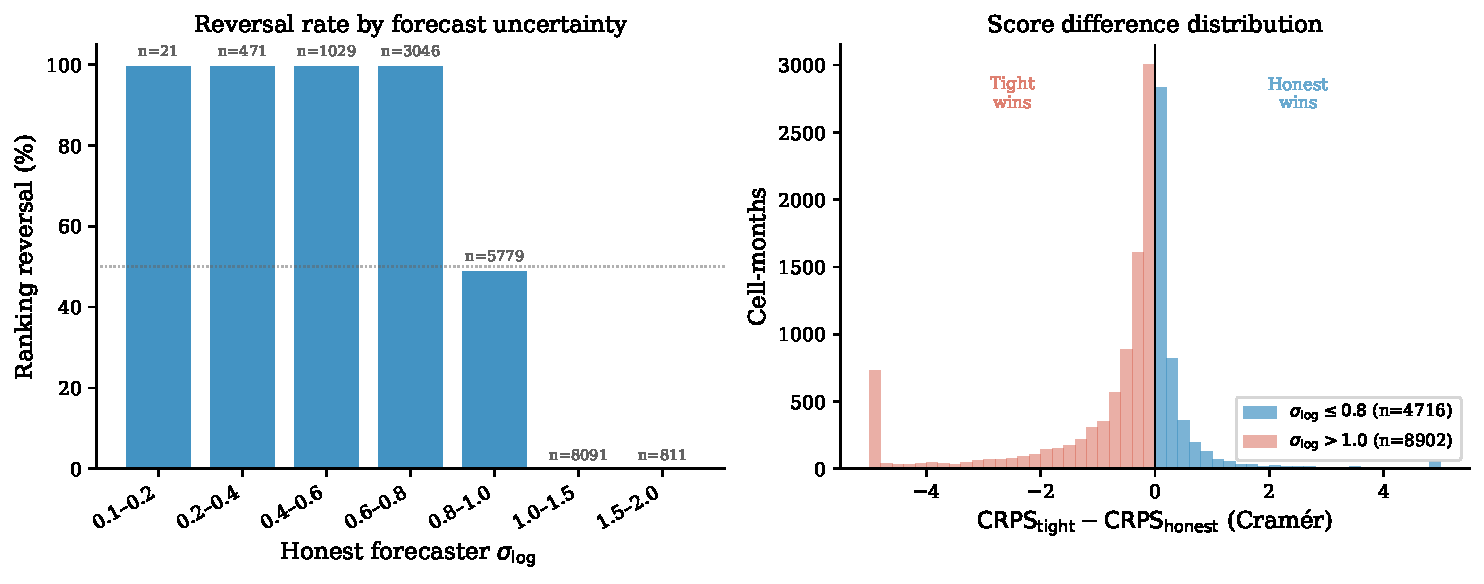
\includegraphics[width=\textwidth]{figures/real_data_comparison.pdf}
    \caption{Ranking reversal on UCDP conflict data (2020--2024, 19{,}397 cell-months). Left: reversal rate under the Cram\'er-distance reformulation as a function of the honest version's log-space uncertainty $\hat{\sigma}_\text{cell}$. The reversal is complete for $\hat{\sigma}_\text{cell} \leq 0.8$ and absent for $\hat{\sigma}_\text{cell} > 1.0$. Right: distribution of score differences; positive values indicate the honest version wins.}
    \label{fig:real_data}
\end{figure}

Among cell-months with genuine UCDP low/best/high bounds, Constructor~1 produces a reversal rate of only 9.9\%---reflecting the fact that UCDP's coding ranges are narrow relative to the true observational uncertainty \citep{vesco2026uncertainty}. Under the RVI Gumbel mixture (Constructor~2), the reversal widens to 80.8\% of cell-months, capturing asymmetric underreporting that the symmetric parametric constructor misses. The Bessac--Naveau conditional-expectation correction \citep{bessac2021forecast} confirms the pattern, with 98.1\% concordance overall. A per-violence-type breakdown, constructor comparison details, and the unit-of-analysis caveat for Constructor~2 are in Appendix~\ref{sec:appendix_demo}.

\subsection{Validation with an operational forecaster}

The preceding comparisons centre both versions on the reported value $y$---information unavailable at prediction time. This isolates the spread effect but leaves open whether the reversal survives when the model does not observe $y$. I test this using HydraNet \citep{VonDerMaase2025hydranet}, a spatio-temporal Monte Carlo Dropout architecture trained on the Violence \& Impacts Early-Warning System (VIEWS) PRIO-GRID. The model produces 64 posterior samples per cell-month\footnote{The HydraNet architecture draws 128 samples per cell-month in its reference configuration; the validation here uses 64 due to local memory constraints.} for each violence type; I use state-based fatalities, the best-documented violence type with the lowest reversal rate in the synthetic comparison (79.3\% under RVI; Appendix~\ref{sec:appendix_demo})---the reformulation's impact is likely larger for non-state and one-sided violence, where observational uncertainty is greater.

\paragraph{Setup.}
The model is trained on January 1990--December 2020 and produces 36-step-ahead validation predictions for January 2021--December 2024 (the standard VIEWS validation partition). I match these against UCDP state-based fatality actuals aggregated to the cell-month level, using the shortest-horizon (most recent) prediction available for each cell-month, yielding 6{,}725 cell-months across 1{,}173 cells where the reported best estimate is positive. For each cell-month, I construct two versions of the same model's output---this tests whether the metric values uncertainty quantification, not whether it changes model selection between genuinely different systems:
\begin{itemize}
    \item \textbf{Full posterior:} the model's 64 posterior samples, used directly as the forecast distribution.
    \item \textbf{Tight:} $\text{LogNormal}(\log \bar{x}, \, 0.05)$ where $\bar{x}$ is the posterior mean---a version that retains the model's location estimate but discards its uncertainty quantification.
\end{itemize}
Both versions share the same location; the only difference is spread.

\paragraph{Results.}
In the full sample, classical CRPS strictly prefers the tight version in only 2.5\% of cell-months (167/6{,}725). A further 16.4\% (1{,}102 cell-months) are ties where the model predicts zero fatalities and both versions are degenerate; the remaining 81.1\% strictly prefer the full posterior. The dominance of the full posterior reflects HydraNet's typically large location errors; when the model misses the location, wider spread helps under classical CRPS simply by placing more mass near the target.

The interesting regime is the 1{,}031 cell-months (15.3\%) where the model's prediction falls within a factor of two of the actual---where location error is moderate and the spread dimension becomes consequential. In this subset, classical CRPS selects the tight version in 167 cell-months (16.2\%). The Cram\'er-distance reformulation (Constructor~3, $\sigma_\text{rel} = 0.4$) reverses 166 of these 167 cases (99.4\%), selecting the full posterior instead. Under the RVI Gumbel constructor (Constructor~2), the reversal rate is 167/167 (100\%). The single cell-month that resists reversal under Constructor~3 is a high-fatality case (best $= 56$) where the full posterior has a log-space standard deviation of $0.77$---genuinely too wide relative to $F_\text{obs}$. The Cram\'er distance does not reward uncertainty indiscriminately but penalises spread that exceeds observational uncertainty, exactly as in the synthetic demonstration.
